\documentclass[11pt]{article}

\usepackage[letterpaper,margin=1in]{geometry}
\usepackage{setspace}
\usepackage{graphicx}
\usepackage{booktabs}
\usepackage{amsmath,amssymb}
\usepackage{float}
\usepackage{hyperref}
\usepackage{indentfirst}

\onehalfspacing
\setlength{\parindent}{1.5em}

\title{Bayesian Hierarchical Analysis of Crop Yield and Biomass in the GRACEnet Data}
\author{Huixin Li, Weidai He, Qihao Zhang}
\date{STAT 431 Final Project}

\begin{document}
\maketitle

\begin{abstract}
This project analyzes crop outcomes from the GRACEnet agricultural data set using Bayesian hierarchical regression. The main research question is how environmental growing-season conditions and agricultural management practices are associated with crop yield while accounting for site-to-site variability. We model grain carbon content and above-ground biomass separately. Both responses are log-transformed, and each model includes fixed effects for nitrogen input, growing-season precipitation, growing-season temperature, crop, tillage, and residue removal, with a random intercept for experimental site. The posterior results show positive associations for nitrogen input and growing-season precipitation, negative associations for growing-season temperature, and substantial site-level heterogeneity. These findings support the use of a hierarchical model because observations from the same site are not exchangeable with observations from other sites. The results also provide quantitative evidence that may help evaluate crop production strategies under different environmental conditions.
\end{abstract}

\section{Introduction}

Crop productivity depends on both environmental conditions and management decisions. In agricultural field experiments, observations are often collected across multiple sites, years, crops, and treatment practices. A standard regression model that treats all observations as independent may underestimate uncertainty because observations from the same site share climate, soil, management history, and experimental design features. The goal of this project is to use a Bayesian hierarchical model to quantify associations between crop outcomes and predictors while allowing different sites to have distinct baseline yield levels.

The analysis follows Option 1 of the project instructions: a Bayesian hierarchical model analysis of a real data set using Markov chain Monte Carlo. The primary response is grain carbon content, measured as kg C/ha, which we use as a yield-related outcome. A secondary response is above-ground biomass, measured as kg/ha. The two outcomes are modeled separately so that the interpretation of each response remains clear.

This analysis is connected to several lines of related work. First, GRACEnet was developed by the USDA Agricultural Research Service to support coordinated, multi-location evaluation of greenhouse gas emissions, soil carbon, crop yields, and agricultural management systems. Jawson et al. describe GRACEnet as a standardized cross-location research network designed to provide empirical evidence for agricultural carbon sequestration and environmental management decisions [1]. The USDA data description similarly emphasizes that the network compares management systems across cropped and grazed soils and includes biomass yield, fertilizer, weather, and land-management information [2]. Second, Bayesian and hierarchical models are widely used when agricultural outcomes vary over space, time, or experimental grouping units. For example, Jiang et al. used a Bayesian spatial hierarchical model to analyze within-field corn yield variability [3], and Saengseedam and Kantanantha used Bayesian MCMC estimation for mixed spatio-temporal crop-yield models [4]. More recent crop-yield work also uses Bayesian spatial or hierarchical models to borrow information across locations and quantify uncertainty in yield prediction [5, 6]. These papers motivate our use of a hierarchical model for GRACEnet observations nested within sites.

\section{Data}

The data come from GRACEnet, the Greenhouse gas Reduction through Agricultural Carbon Enhancement network, compiled by the USDA Agricultural Research Service [2]. The data file used here contains 5,781 observations from 11 site identifiers, with years ranging from 1990 to 2015. The median number of observations per site is 100, with site sizes ranging from 12 to 3,104 observations. The geographic distribution of the 11 sites based on their latitude and longitude coordinates is shown in Figure 1.

% === Add the map ===
\begin{figure}[H]
\centering
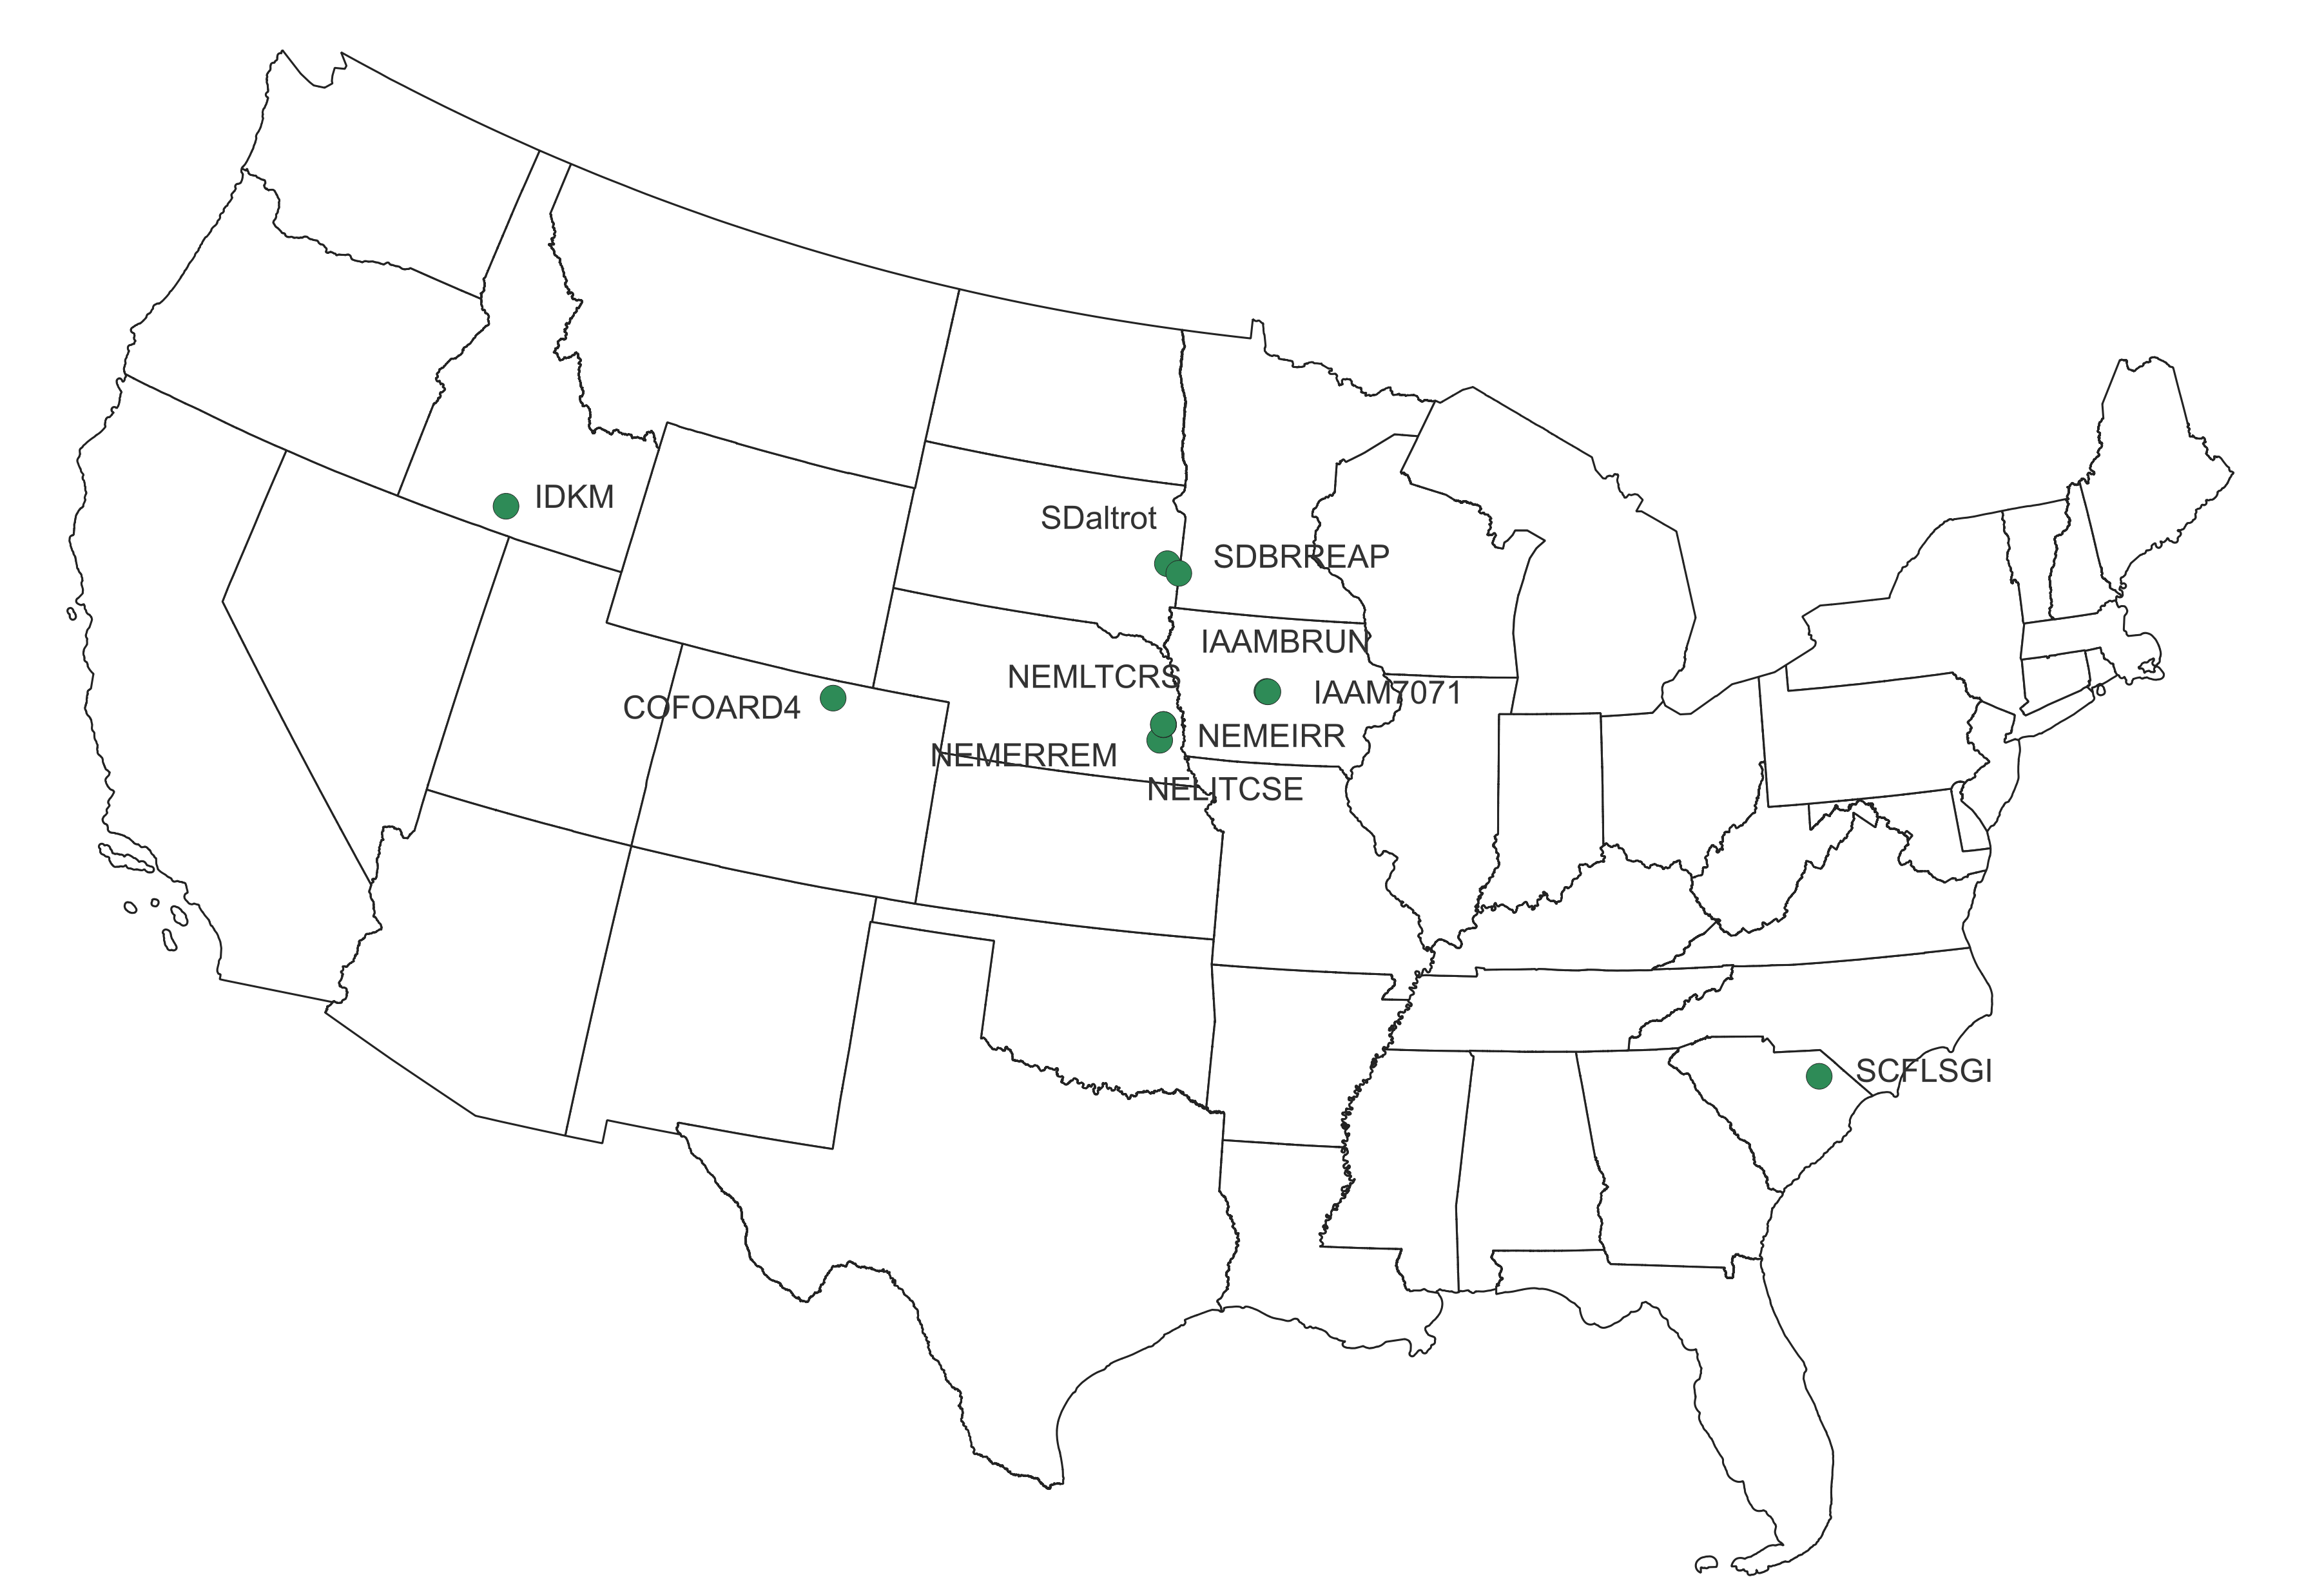
\includegraphics[width=0.75\textwidth]{outputs/figures/gracenet_site_map.png}
\caption{Location of GRACEnet experimental sites across the United States.}
\label{fig:site-map}
\end{figure}

Table \ref{tab:variables} summarizes the variables used in the final model. The variables \texttt{GS\_P} and \texttt{GS\_T} summarize growing-season conditions: \texttt{GS\_P} is total precipitation during the growing season, and \texttt{GS\_T} is average growing-season temperature. These variables represent important temporal and environmental variation, so year is reported descriptively but is not used as a second hierarchical level in the final model.

\begin{table}[H]
\centering
\caption{Variables used in the analysis}
\label{tab:variables}
\begin{tabular}{llll}
\toprule
Variable & Unit & Role & Meaning \\
\midrule
Grain C & kg C/ha & Primary response & Grain carbon content \\
Above-ground biomass & kg/ha & Secondary response & Above-ground crop biomass \\
SiteID & - & Grouping variable & Experimental site \\
Crop & - & Categorical predictor & Crop species \\
Tillage descriptor & - & Categorical predictor & Tillage management class \\
Residue removal & - & Categorical predictor & Residue removal category \\
Total N amount & kg N/ha & Continuous predictor & Annual nitrogen application \\
GS\_P & mm & Continuous predictor & Growing-season precipitation \\
GS\_T & degrees C & Continuous predictor & Growing-season temperature \\
\bottomrule
\end{tabular}
\end{table}

The main crop categories are corn and soybean: 4,021 observations are corn and 1,738 are soybean. The remaining crop categories are much smaller: barley has 12 observations, pea has 5, and winter wheat has 5. The tillage categories are conventional tillage (3,848), no tillage (940), conservation tillage (645), sub tillage (201), and strip tillage (147). Residue removal is mostly ``No'' (4,849), with 561 partial-removal observations and 371 removal observations.

\section{Data Processing and Descriptive Analysis}

Missingness was an important part of the data-processing decision. Cover crop, sand percentage, clay percentage, and organic carbon had more than 90\% missing values, so they were not included in the final model. Soil pH was missing for about 32\% of observations, and including it would have removed a large fraction of the data. The final model therefore focuses on variables with stronger coverage: nitrogen input, growing-season precipitation, growing-season temperature, crop, tillage, residue removal, and site.

The response variables are positive and right-skewed, so both grain carbon and biomass are modeled on the log scale. This transformation makes the Gaussian likelihood more appropriate and gives regression coefficients an approximate multiplicative interpretation on the original scale. Continuous predictors are standardized before modeling. After dropping observations with missing model variables, the grain-carbon model uses 4,969 observations, and the biomass model uses 4,527 observations.

\begin{table}[H]
\centering
\caption{Selected descriptive summaries for continuous variables}
\label{tab:descriptive}
\begin{tabular}{llllll}
\toprule
Variable & Unit & Mean & SD & Median & Range \\
\midrule
Grain C & kg C/ha & 2637.94 & 1333.60 & 2546.89 & 38.36--7703.29 \\
Biomass & kg/ha & 11737.75 & 5393.45 & 11360.44 & 703.33--30946.11 \\
Total N & kg N/ha & 109.14 & 81.01 & 112.00 & 0.00--1064.00 \\
GS\_P & mm & 462.78 & 216.30 & 461.01 & 0.00--963.42 \\
GS\_T & degrees C & 19.46 & 1.70 & 19.45 & -2.55--25.81 \\
\bottomrule
\end{tabular}
\end{table}

\begin{figure}[H]
\centering
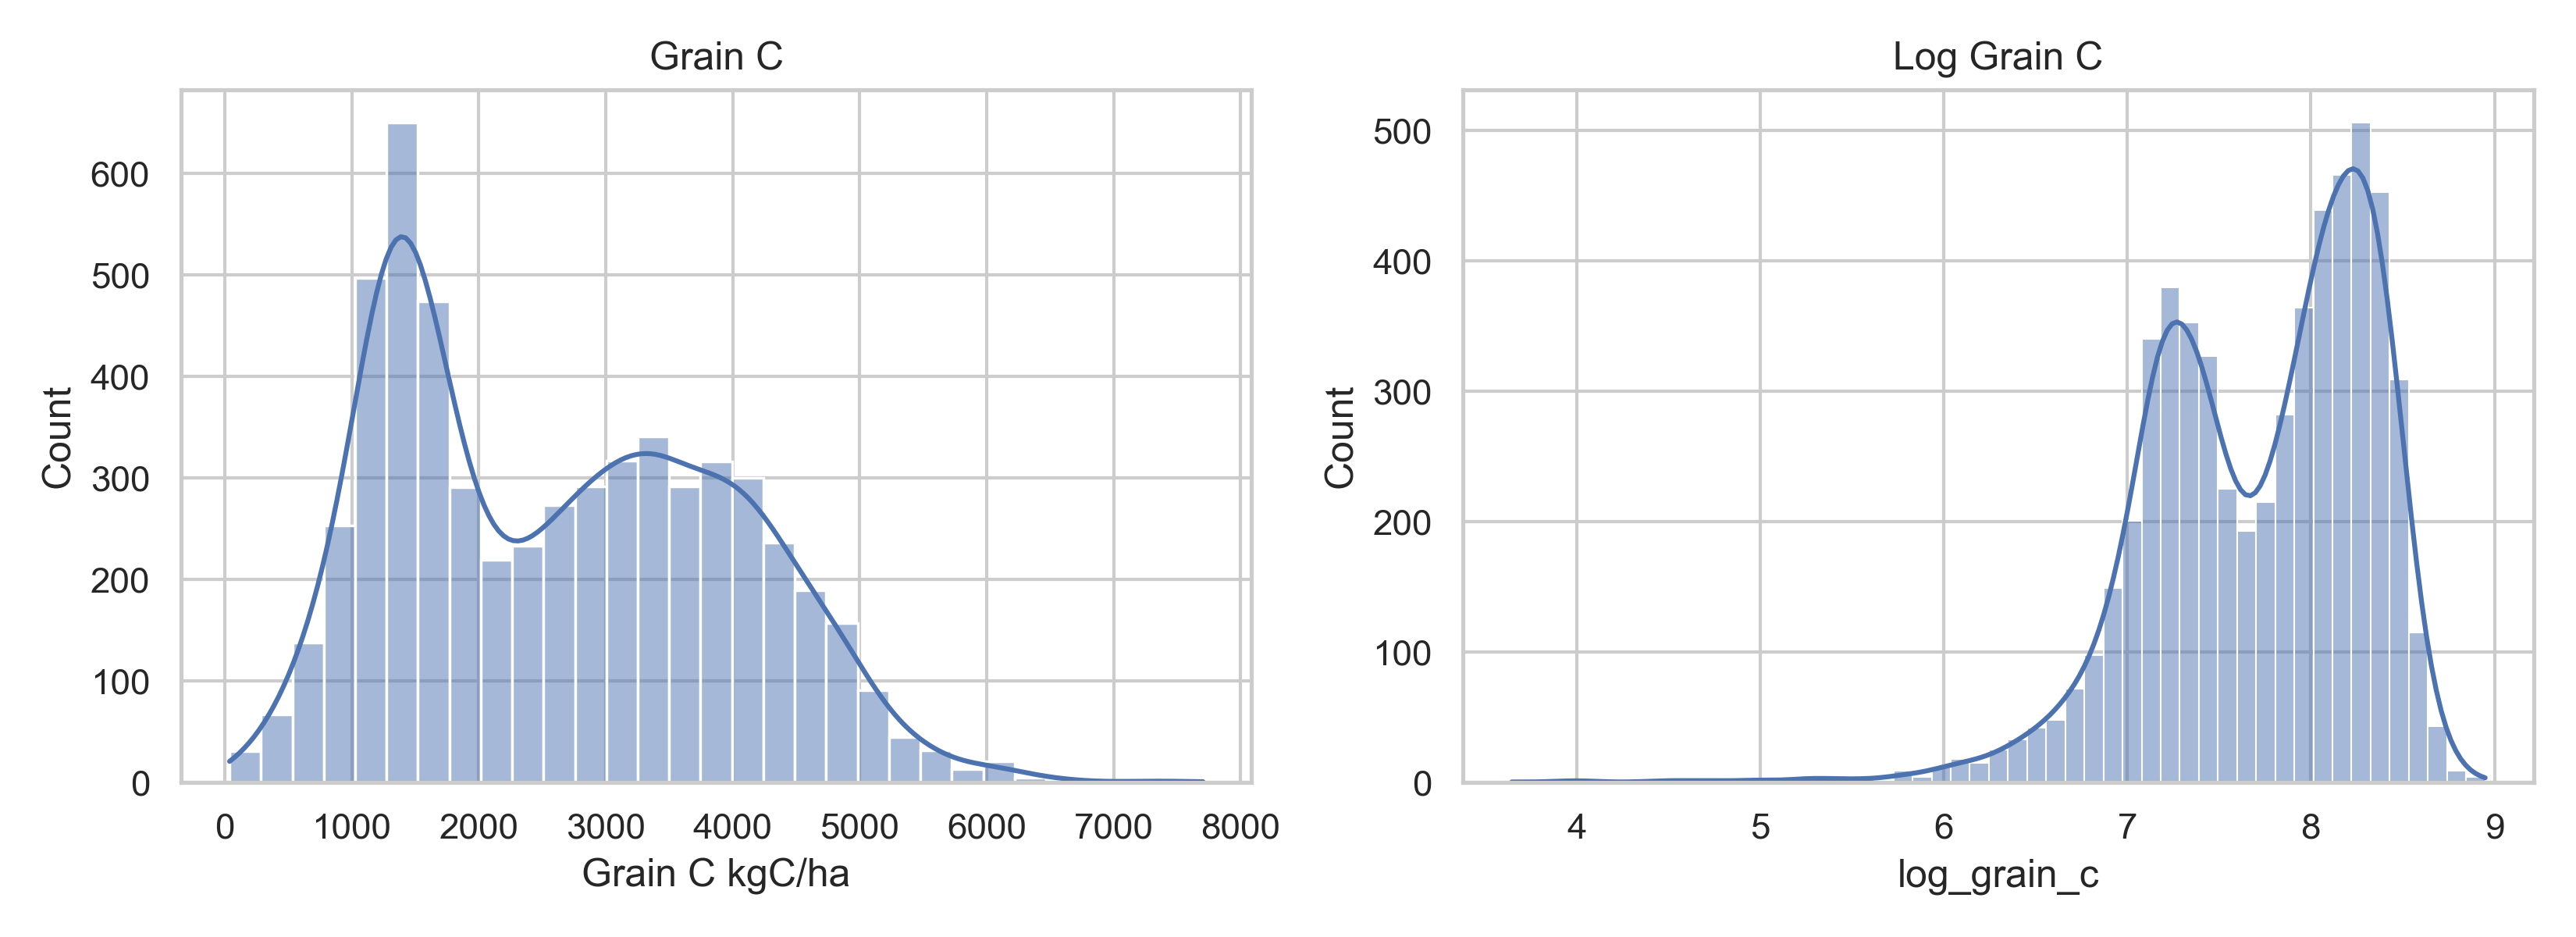
\includegraphics[width=0.82\textwidth]{outputs/figures/grain_c_distribution.png}
\caption{Distribution of grain carbon before and after log transformation}
\label{fig:grain-dist}
\end{figure}

\begin{figure}[H]
\centering
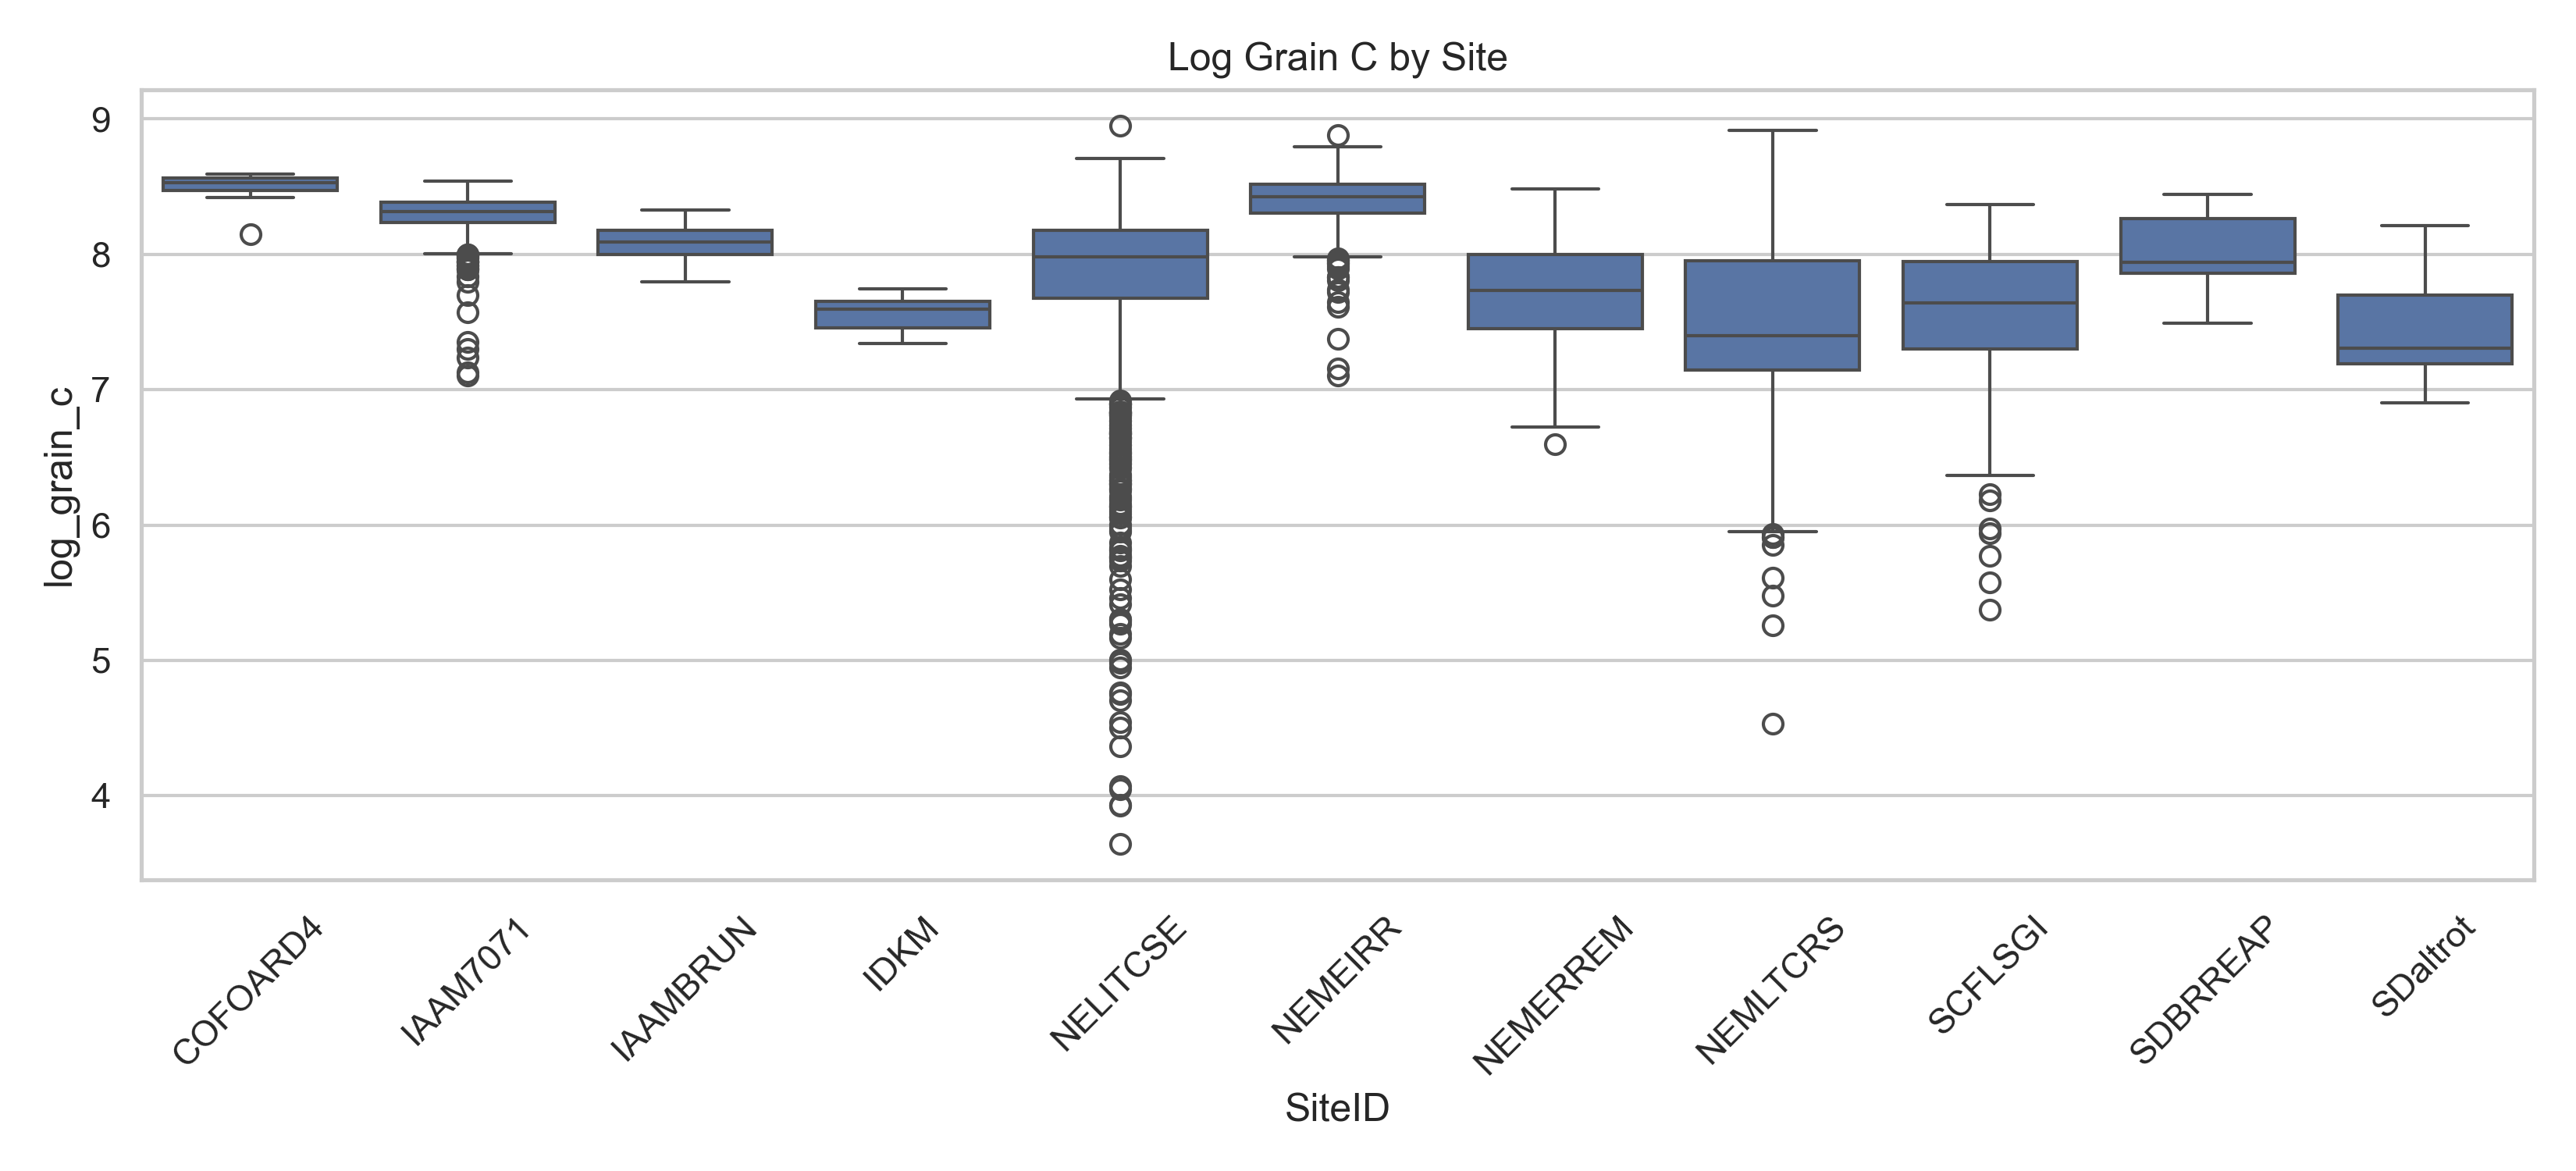
\includegraphics[width=0.82\textwidth]{outputs/figures/log_grain_c_by_site.png}
\caption{Log grain carbon by site. The visible site-to-site differences motivate a hierarchical model with random site intercepts}
\label{fig:site-box}
\end{figure}

\section{Methods and Methodological Justification}

The analysis uses a Bayesian hierarchical linear regression model. This choice is appropriate for three reasons. First, the data have a grouped structure: observations are nested within sites, and sites differ in climate, soil, experimental design, and management history. Multilevel or hierarchical models are designed for this kind of grouped data because they allow partial pooling, a compromise between complete pooling and no pooling, across groups [7, 8]. In this project, partial pooling is especially useful because site sizes are highly unbalanced, ranging from 12 to 3,104 observations. Under partial pooling, site estimates are allowed to differ, but smaller or noisier site-specific estimates are shrunk toward the overall mean, with the amount of shrinkage depending on site sample size and the estimated between-site variance.

Second, Bayesian inference gives direct posterior uncertainty statements for regression coefficients, variance components, and site-level heterogeneity. This is useful for the project question because the goal is not only to estimate associations, but also to quantify uncertainty in environmental and management effects. The Bayesian framework also gives a coherent way to include weakly informative priors, which regularize estimates for small or imbalanced categorical groups.

Third, MCMC is a standard computational tool for Bayesian hierarchical models when posterior distributions are not available in closed form. We use a Gibbs sampler because, under a Gaussian likelihood with normal priors for regression and random-effect terms and inverse-gamma priors for variance components, the full conditional distributions have standard forms. This makes the sampler transparent and easy to document in the appendix. Following the convergence-diagnostic strategy of Gelman and Rubin, we run multiple chains and summarize convergence using trace plots and $\hat{R}$ [9].

The log transformation is used because grain carbon and biomass are positive, right-skewed agricultural outcomes. Modeling the log response improves compatibility with a Gaussian error model and makes coefficients interpretable as approximate proportional changes on the original scale. Similar log-transformed mixed models have been considered in crop-yield forecasting settings where yield distributions are skewed or heterogeneous [4].

\section{Bayesian Hierarchical Model}

Let $i=1,\ldots,n$ index observations and let $j[i]$ denote the site for observation $i$. For the grain-carbon analysis, the response is
\[
y_i = \log(\text{Grain C}_{i}).
\]
For the biomass analysis, the same model is used with
\[
y_i = \log(\text{Above-ground Biomass}_{i}).
\]
Let $x_i$ be the row vector of fixed-effect predictors, including an intercept, standardized nitrogen input, standardized growing-season precipitation, standardized growing-season temperature, and dummy variables for crop, tillage, and residue removal. Conservation tillage, soybean, and no residue removal are the baseline categories when those categories are present in the model matrix.

The model is
\begin{align*}
y_i \mid \beta, a_{j[i]}, \sigma^2
  &\sim \text{Normal}(x_i^\top \beta + a_{j[i]}, \sigma^2),\\
a_j \mid \tau^2
  &\sim \text{Normal}(0,\tau^2), \qquad j=1,\ldots,J,\\
\beta_k
  &\sim \text{Normal}(0,10^2),\\
\sigma^2
  &\sim \text{Inverse-Gamma}(2,1),\\
\tau^2
  &\sim \text{Inverse-Gamma}(2,1).
\end{align*}
Here $a_j$ is the random intercept for site $j$, $\sigma$ is the observation-level residual standard deviation, and $\tau$ is the between-site standard deviation. The priors are weakly informative on the log-response scale. They regularize the model while leaving the data to dominate the posterior for the main coefficients.

In matrix form, the fitted model can be written as $y = X\beta + Za + \epsilon$. Here $X$ is an $n \times p$ fixed-effect design matrix containing the intercept, three standardized continuous predictors, and dummy variables for crop, tillage, and residue removal. The value of $p$ depends on which categorical levels remain after complete-case filtering; in the implemented analysis, $p=14$ for the grain-carbon model and $p=12$ for the biomass model. The matrix $Z$ is an $n \times J$ site-indicator matrix, where $J=10$ for the grain-carbon complete-case data and $J=7$ for the biomass complete-case data.

\section{Computation}

The analysis was implemented with two Python scripts. The first script, \texttt{project\_analysis.py}, performs the non-MCMC preparation steps. It reads \texttt{gracenet\_data.csv}, treats \texttt{NA} values as missing, converts site and management variables to categorical variables, creates the log-transformed responses, standardizes the continuous predictors, and writes summary tables for missingness, site sizes, year ranges, categorical counts, and numeric descriptive statistics. It also creates exploratory figures, including the response distributions and the site-level boxplot. Finally, it fits preliminary frequentist mixed-effect models with site random intercepts. These preliminary models were used as a model check and comparison point, but the Bayesian posterior results in this report come from the MCMC script.

The second script, \texttt{mcmc\_\allowbreak hierarchical\_\allowbreak model.py}, implements the Bayesian hierarchical model by Gibbs sampling. For each response, the script constructs the response vector $y$, a fixed-effect design matrix $X$ containing an intercept, standardized continuous predictors, and dummy-coded categorical predictors, and a site index vector for the random intercepts. The site index is converted into a site-design matrix $Z$, so the linear predictor can be written as $X\beta + Za$. The script then runs four independent MCMC chains using different random seeds.

Posterior inference was performed using this Gibbs sampler. Conditional on the variance parameters, the fixed effects and site random effects have a multivariate normal full conditional distribution, so the script samples $\beta$ and $a$ jointly from a multivariate normal distribution. The residual variance $\sigma^2$ and site-level variance $\tau^2$ have inverse-gamma full conditional distributions and are sampled directly from those distributions. Four independent chains were run for each response. Each chain used 3,500 iterations with the first 1,000 discarded as burn-in, leaving 10,000 post-burn-in posterior draws per response across all chains.

After sampling, \texttt{mcmc\_\allowbreak hierarchical\_\allowbreak model.py} combines the post-burn-in draws across chains and writes posterior means, posterior standard deviations, 2.5\%, 50\%, and 97.5\% posterior quantiles, and $\hat{R}$ diagnostics to CSV files. It also creates trace plots for the intercept, nitrogen input, growing-season precipitation, growing-season temperature, residual standard deviation, and site-level standard deviation. The main output files used in the report are the posterior summary CSV files for log grain carbon and log biomass, plus the corresponding MCMC trace plots in the \texttt{outputs/figures/} directory.

Convergence was evaluated using trace plots and the potential scale reduction factor $\hat{R}$. For the main parameters in both models, $\hat{R}$ values were approximately 1.00, indicating no visible evidence of non-convergence.

\begin{figure}[H]
\centering
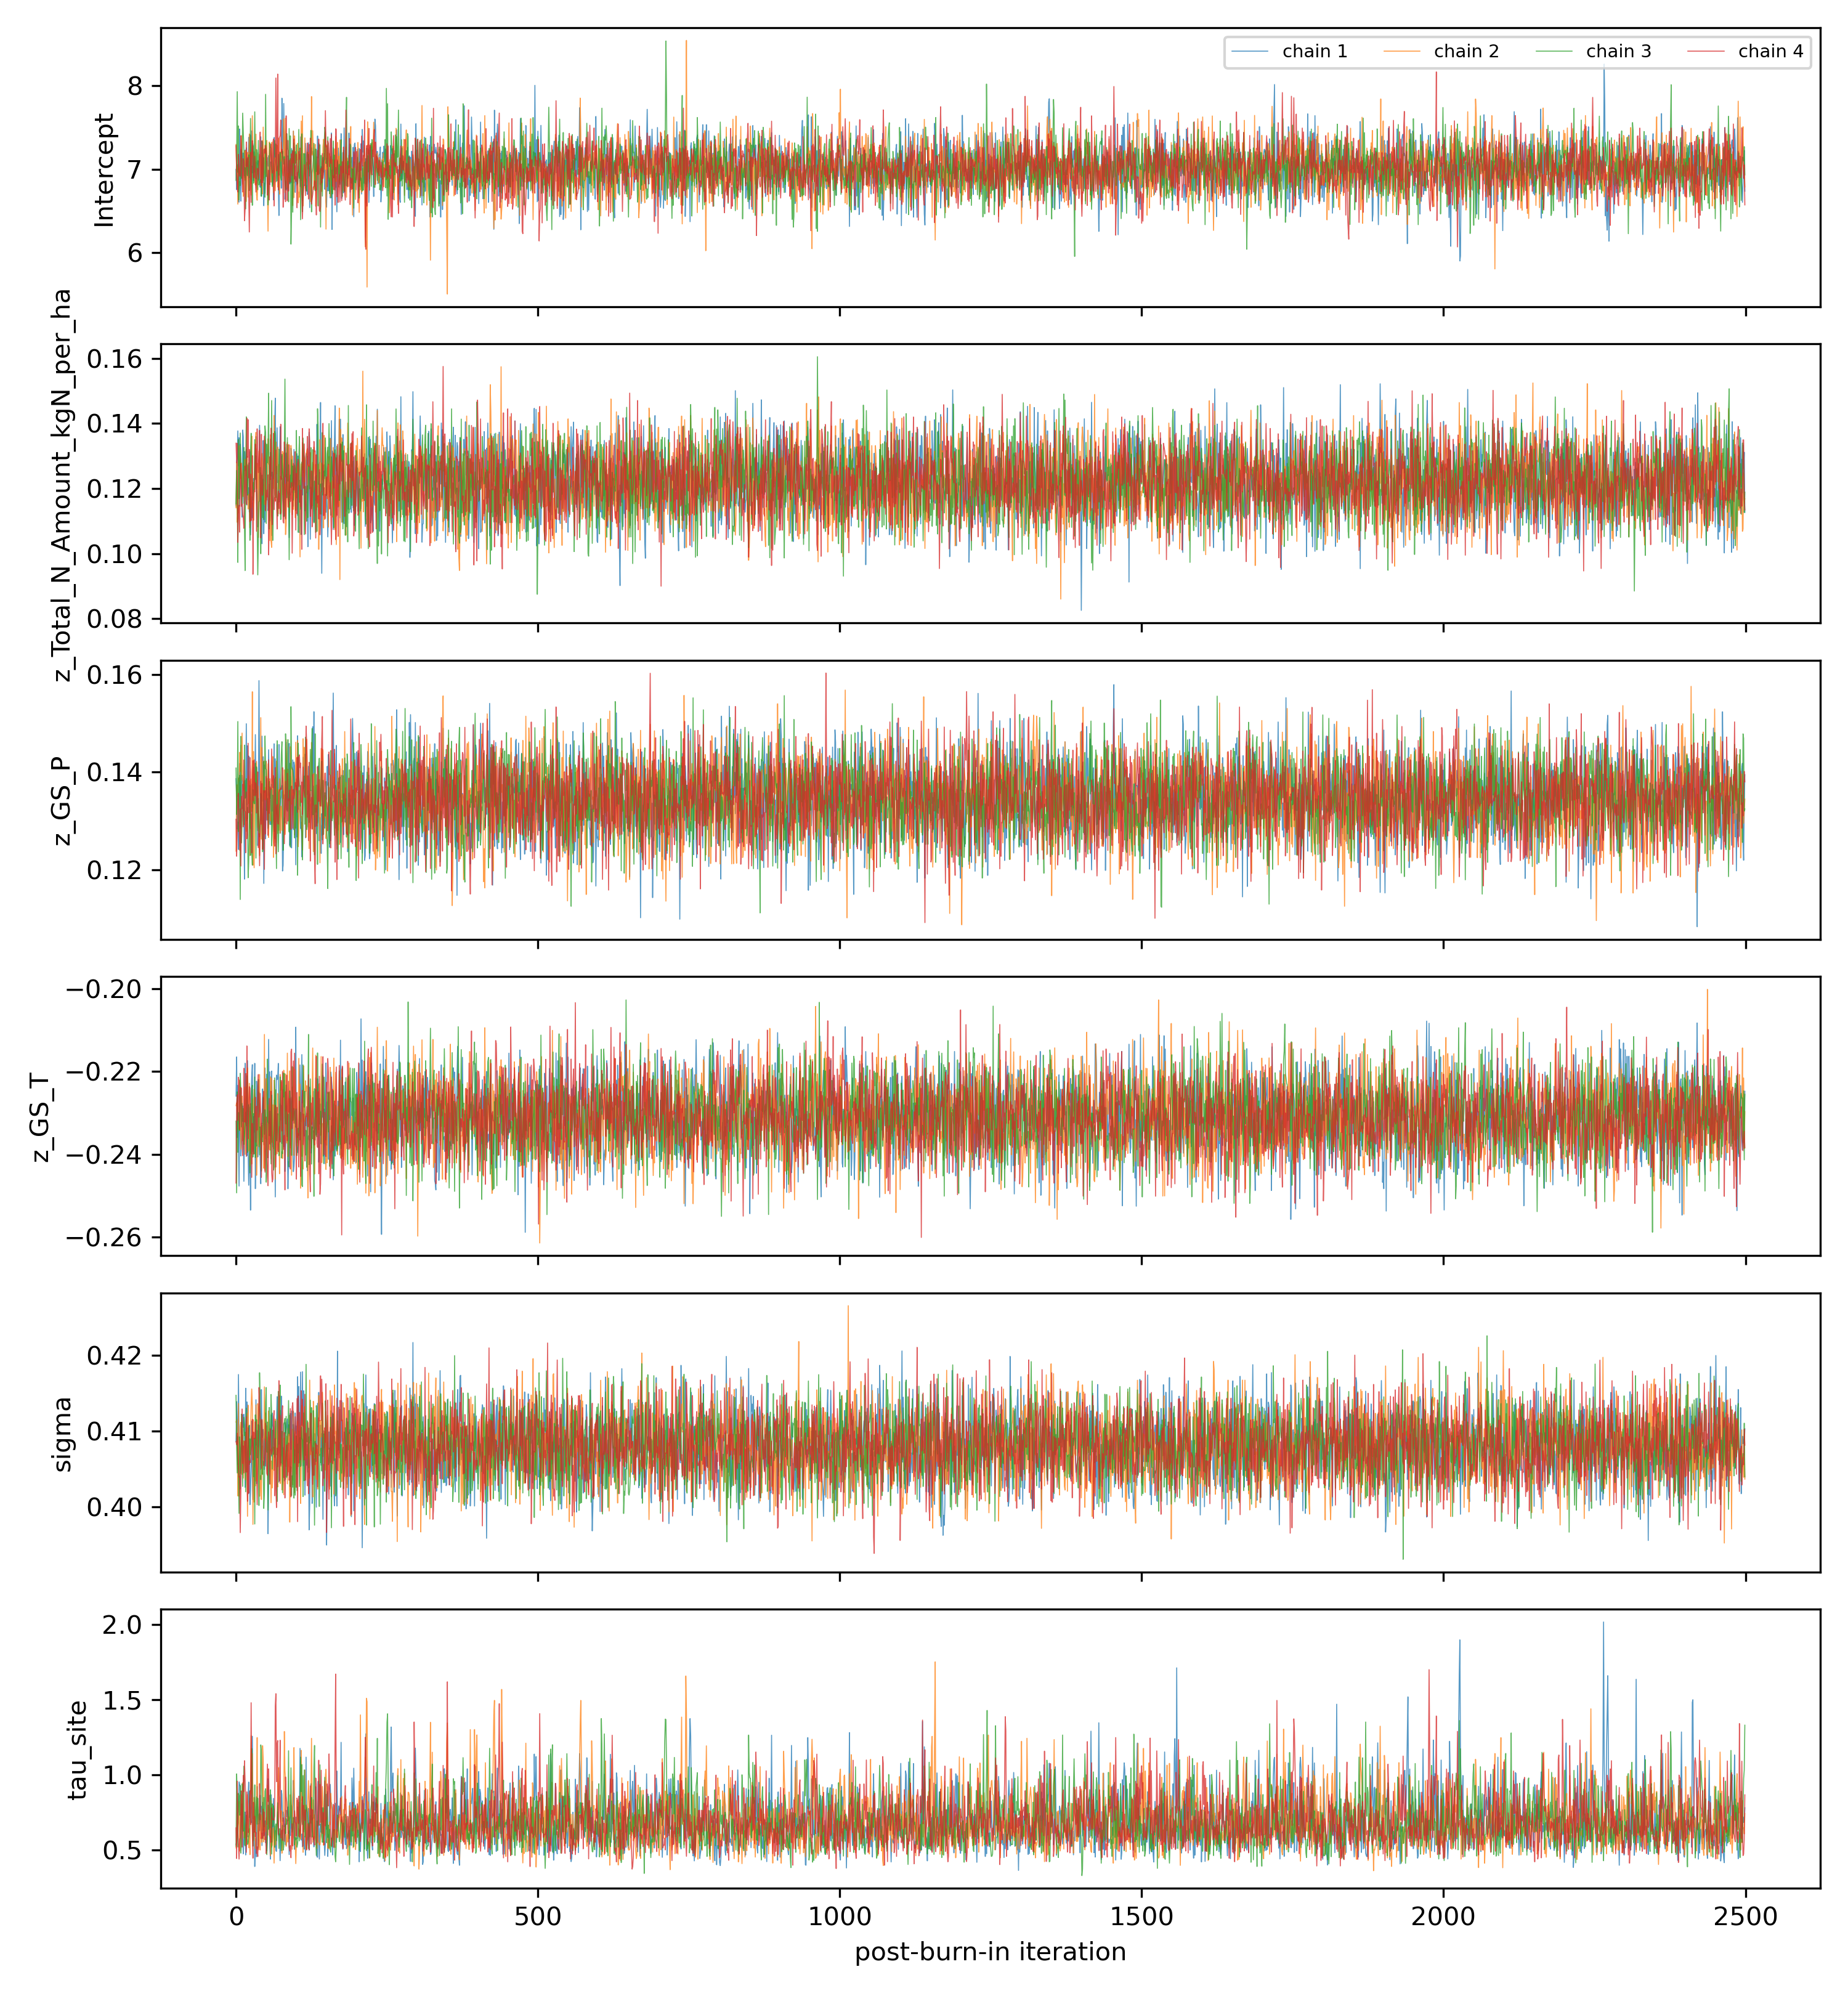
\includegraphics[width=0.58\textwidth,trim=25 35 25 35,clip]{outputs/figures/log_grain_c_mcmc_trace.png}
\caption{Trace plots for selected grain-carbon model parameters}
\label{fig:grain-trace}
\end{figure}

\section{Results}

Table \ref{tab:grain-post} gives posterior summaries for the main grain-carbon model parameters. Since continuous predictors are standardized, the coefficients represent the expected change in log grain carbon for a one-standard-deviation increase in the predictor, holding the other variables fixed.

\begin{table}[H]
\centering
\caption{Posterior summaries for selected grain-carbon model parameters}
\label{tab:grain-post}
\begin{tabular}{lrrrr}
\toprule
Parameter & Mean & SD & 95\% CrI & $\hat{R}$ \\
\midrule
Nitrogen input & 0.122 & 0.010 & [0.103, 0.141] & 1.000 \\
GS\_P & 0.134 & 0.007 & [0.121, 0.148] & 1.000 \\
GS\_T & -0.231 & 0.008 & [-0.247, -0.216] & 1.000 \\
Corn vs. soybean & 0.569 & 0.017 & [0.536, 0.603] & 1.001 \\
Conventional tillage & 0.056 & 0.026 & [0.006, 0.107] & 1.000 \\
No till & 0.040 & 0.026 & [-0.011, 0.090] & 1.000 \\
Sub till & -0.070 & 0.035 & [-0.139, -0.001] & 1.000 \\
Residual SD $\sigma$ & 0.408 & 0.004 & [0.400, 0.416] & 1.000 \\
Site SD $\tau$ & 0.690 & 0.168 & [0.452, 1.095] & 1.000 \\
\bottomrule
\end{tabular}
\end{table}

For grain carbon, nitrogen input and growing-season precipitation both have positive posterior associations. The 95\% credible interval for nitrogen is [0.103, 0.141], and the interval for growing-season precipitation is [0.121, 0.148]. Because both predictors are standardized, these effects compare observations that differ by one sample standard deviation in the predictor while holding the other model terms fixed. On the original grain-carbon scale, the nitrogen coefficient of 0.122 corresponds to an approximate $\exp(0.122)-1=13.0\%$ increase in expected grain carbon for a one-standard-deviation increase in nitrogen input. The growing-season precipitation coefficient of 0.134 corresponds to an approximate 14.4\% increase. The fact that both credible intervals are entirely above zero indicates strong posterior evidence that these predictors are positively associated with grain carbon in this model. In practical terms, these estimates suggest that improved nitrogen availability and favorable growing-season water conditions are associated with meaningfully higher yield-related carbon output.

Growing-season temperature has a negative association with grain carbon. Its posterior mean is $-0.231$, with a 95\% credible interval of [$-0.247$, $-0.216$]. On the original scale, this is approximately a 20.6\% decrease in expected grain carbon for a one-standard-deviation increase in growing-season temperature, after adjusting for nitrogen, precipitation, crop, tillage, residue removal, and site. This result should be interpreted as an adjusted association rather than a causal temperature effect, because the data combine multiple sites and experimental contexts. Still, the posterior interval is narrow and fully below zero, so the direction of the association is stable under the fitted model.

The crop coefficient for corn relative to soybean is also large and positive. The posterior mean is 0.569, corresponding to an approximate 76.7\% higher expected grain-carbon response for corn than soybean, conditional on the other predictors. This reflects the strong biological and production differences between the main crop groups in the data. In contrast, the smaller crop categories have wide credible intervals because barley, pea, and winter wheat have very few observations. Their posterior summaries should therefore not be overinterpreted.

The tillage and residue-removal effects are more modest. Conventional tillage has a small positive association with grain carbon, with posterior mean 0.056 and a 95\% credible interval [0.006, 0.107]. No tillage and residue-removal categories have intervals that include zero, so the posterior evidence for those effects is weaker after adjusting for the other variables. Sub tillage has a small negative posterior mean, with its interval barely below zero. This suggests that the management effects are less uniform than the environmental predictors and may depend on site-specific or crop-specific contexts that are not fully represented by the current model.

The posterior mean for the site-level standard deviation is 0.690, with a 95\% credible interval of [0.452, 1.095]. This is large relative to several fixed-effect coefficients and confirms that between-site variation is an important part of the data. Since $\exp(0.690) \approx 1.994$, a site effect of this magnitude corresponds to approximately a 99.4\% increase, nearly a doubling, on the original scale. The random intercepts are therefore not just a technical adjustment; they capture meaningful baseline differences among sites. The model directly addresses the main dependence structure identified in the proposal: observations are nested within sites, and those sites have different baseline productivity levels.

The biomass model gives similar directional conclusions for the main environmental and management variables. Nitrogen input has posterior mean 0.128 with a 95\% credible interval [0.112, 0.144], corresponding to an approximate 13.7\% increase in expected biomass for a one-standard-deviation increase in nitrogen. Growing-season precipitation has posterior mean 0.085 with interval [0.074, 0.096], corresponding to an approximate 8.8\% increase. Growing-season temperature has posterior mean $-0.131$ with interval [$-0.143$, $-0.120$], corresponding to an approximate 12.3\% decrease. The precipitation association is smaller for biomass than for grain carbon, which may be reasonable because total above-ground biomass includes non-grain plant material and may be less sensitive than grain production to water availability during grain filling. The posterior mean for the site-level standard deviation is 0.508, again indicating site-level heterogeneity. The similarity between the grain-carbon and biomass models strengthens the main conclusion: nitrogen and precipitation are positively associated with crop outcomes, temperature is negatively associated, and site-level differences remain important even after adjusting for observed predictors.

\section{Discussion}

The results suggest that crop outcomes in this data set are associated with both management practices and growing-season environmental conditions. Higher nitrogen input is associated with greater grain carbon and above-ground biomass production because nitrogen directly supports leaf development and photosynthetic activity in cropping systems. Higher growing-season precipitation is also associated with higher biomass and yield, indicating that water availability is an important limitation for carbon assimilation and plant growth, especially in rainfed systems. In contrast, higher growing-season temperature is associated with lower outcomes after controlling for the other predictors, potentially because excessive heat  increases evapotranspiration and accelerate physiological maturity and senescence. Corn shows a much higher expected response than soybean on the log scale. Soybean can partially obtain nitrogen through symbiotic nitrogen fixation, whereas corn lacks this capacity and is therefore more directly constrained by soil-available nitrogen and more responsive to fertilizer management.

The hierarchical model is important because the data are strongly unbalanced across sites. One site contributes more than 3,000 observations while the smallest site contributes only 12. A complete-pooling model would ignore site-level dependence, while a no-pooling model would estimate each site separately and lose information for smaller sites. The Bayesian hierarchical model provides partial pooling: site effects are estimated separately but regularized through the common site-level variance parameter [7]. This shrinkage is especially helpful for small sites because their site effects are estimated with less information and are therefore pulled more strongly toward the overall mean.

Several limitations should be considered. First, this is an observational analysis of compiled experimental data, so posterior associations should not be interpreted as causal effects without stronger assumptions about treatment assignment and site design. Second, several potentially important soil variables had high missingness and were excluded from the final model. Third, the crop categories are highly imbalanced, so estimates for small crop groups such as barley, pea, and winter wheat are uncertain. Fourth, the model assumes linear relationships between the predictors and the log-transformed responses. Residual plots should be examined in future work to assess this assumption. The random site effects are also assumed to be normally distributed, and Q-Q plots of estimated site-level effects would provide an additional model check.

\section{Conclusion}

This analysis used Bayesian hierarchical regression to study GRACEnet crop outcomes while accounting for site-to-site variability. The posterior results show positive associations of nitrogen input and growing-season precipitation with grain carbon and biomass, a negative association with growing-season temperature, and meaningful between-site heterogeneity. These results answer the main research question by showing that both environmental conditions and management practices are related to crop outcomes, and that a hierarchical model is appropriate for quantifying uncertainty across experimental sites. Future work could extend the model by adding spatial correlation structures for geographic proximity, year-level temporal components for long-term trends, or multiple-imputation and measurement-error approaches for soil variables with high missingness.

\clearpage
\section*{References}

\begin{enumerate}
\renewcommand{\labelenumi}{[\theenumi]}
\setlength{\itemsep}{0pt}
\setlength{\parskip}{0pt}

\item Jawson, M. D., Shafer, S. R., Franzluebbers, A. J., Parkin, T. B., and Follett, R. F. (2005). GRACEnet: Greenhouse gas reduction through agricultural carbon enhancement network. \textit{Soil and Tillage Research}, 83, 167--172. \url{https://doi.org/10.1016/j.still.2005.02.015}

\item USDA Agricultural Research Service. (2015). \textit{GRACEnet (Greenhouse gas Reduction through Agricultural Carbon Enhancement network)}. Agricultural Research Service. \url{https://doi.org/10.15482/USDA.ADC/1235557}

\item Jiang, P., Thelen, K. D., Kitchen, N. R., Sudduth, K. A., and Drummond, S. T. (2009). Bayesian analysis of within-field variability of corn yield using a spatial hierarchical model. \textit{Precision Agriculture}, 10, 111--127. \url{https://doi.org/10.1007/s11119-008-9070-4}

\item Saengseedam, P., and Kantanantha, N. (2017). Spatio-temporal model for crop yield forecasting. \textit{Journal of Applied Statistics}, 44(3), 427--440. \url{https://doi.org/10.1080/02664763.2016.1174197}

\item Ramsey, A. F. (2020). Probability distributions of crop yields: A Bayesian spatial quantile regression approach. \textit{American Journal of Agricultural Economics}, 102(1), 220--239. \url{https://doi.org/10.1093/ajae/aaz029}

\item Park, Y., Li, B., and Li, Y. (2023). Crop yield prediction using Bayesian spatially varying coefficient models with functional predictors. \textit{Journal of the American Statistical Association}, 118(541), 70--83. \url{https://doi.org/10.1080/01621459.2022.2123333}

\item Gelman, A., and Hill, J. (2007). \textit{Data Analysis Using Regression and Multilevel/Hierarchical Models}. Cambridge University Press.

\item Gelman, A., Carlin, J. B., Stern, H. S., Dunson, D. B., Vehtari, A., and Rubin, D. B. (2013). \textit{Bayesian Data Analysis} (3rd ed.). Chapman and Hall/CRC. \url{https://doi.org/10.1201/b16018}

\item Gelman, A., and Rubin, D. B. (1992). Inference from iterative simulation using multiple sequences. \textit{Statistical Science}, 7(4), 457--472. \url{https://doi.org/10.1214/ss/1177011136}

\end{enumerate}

\clearpage
\section*{Appendix}

\subsection*{Contributions}

Huixin Li contributed to project framing, data cleaning, exploratory summaries, data interpretation, interpretation of agricultural variables, and report writing. Weidai He and Qihao Zhang jointly contributed to data cleaning, model implementation, MCMC computation, figure generation, and report writing. All group members reviewed the final project materials.

\subsection*{AI Acknowledgment}

This project used generative AI assistance (ChatGPT) during the coding and report-development process.

For the coding portion, AI assistance was used in three main ways. First, AI helped suggest the overall structure of the analysis workflow, including separating the project into one script for data preparation and exploratory analysis and another script for Bayesian MCMC. Second, AI helped provide template code structures for reading the GRACEnet data, creating summary tables and exploratory figures, setting up the hierarchical model design matrices, and organizing MCMC output files. Third, AI helped identify and fix coding issues during development, including debugging data-preparation steps, correcting missing-column problems, improving comments, and checking that the scripts could run without syntax errors.

For the LaTeX report, the group provided the overall written explanation, the intended analysis results, the mathematical notation for the model, and the figures that should be included in the report. AI assistance was used mainly to convert this material into a polished LaTeX format, organize the section structure, format the provided mathematical notation, insert tables and figures, and adjust the layout of the final PDF. The group reviewed the generated code, outputs, and written explanations and remains responsible for the final analysis decisions, interpretations, and submitted work.

\subsection*{Code Availability}
The complete code for this project is available on GitHub: 
\url{https://github.com/qihao-2/Bayesian-Hierarchical-Analysis-of-Crop-Yield-and-Biomass-in-the-GRACEnet-Data-coding}.

The main analysis files are \texttt{project\_analysis.py} and \texttt{mcmc\_\allowbreak hierarchical\_\allowbreak model.py}. The first script creates variable summaries, missingness tables, descriptive statistics, exploratory figures, and preliminary mixed-model summaries. The second script implements the Gibbs sampler used for posterior inference in the Bayesian hierarchical models. Output tables and figures are written to the \texttt{outputs/} directory. The analysis was run with Python 3.12.3. Required Python packages include \texttt{numpy} 1.26.4, \texttt{pandas} 2.2.2, \texttt{matplotlib} 3.9.2, \texttt{seaborn} 0.13.2, and \texttt{statsmodels} 0.14.2. On the current machine, the MCMC script takes about 10--25 seconds to run depending on system load.

\end{document}
